\chapter{State of the Art}\label{cha:stateoftheart}


	The framework is based on identifying resources by using Uniform Resource Identifiers (URIs), and describing them in terms of properties and property values, which enables to represent statements about resources as a graph of nodes and arcs formed by the resources, their properties and their property values. For example, in figure \ref{fig:rdfexample} we can find a RDF graph representing a person named Eric Miller. Note that the resources itself as well as the properties and property values may be identified by URIs.
	\begin{figure}
	  \centering
	  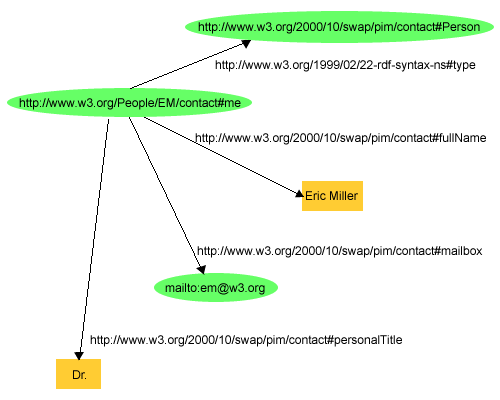
\includegraphics[width=.5\textwidth]{fig/rdfexample}
	  \caption{An RDF graph representing Eric Miller}
	  \captionsetup{font={footnotesize,bf,it}}
	  \caption*{source: \url{http://www.w3.org/TR/2004/REC-rdf-primer-20040210}}
	  \label{fig:rdfexample}
	\end{figure}
